\documentclass{beamer}

% german content
\usepackage[ngerman]{babel}
\usepackage{fontspec}

\setmonofont{FuraCode Nerd Font Mono}
\usepackage[newfloat]{minted}
\SetupFloatingEnvironment{listing}{name=Listing}
\newminted{shell}{
  linenos,
  numbersep=6pt,
  frame=lines,
  framesep=2mm,
  fontsize=\footnotesize
}

% images
\usepackage{graphicx}
\graphicspath{ {./images/} }

\title{Kolloquium zur Bachelorarbeit}
\subtitle{Entwicklung und Evaluation von Methoden zur Absenkung der Nutzungsschwelle von Kommandozeilen-Interfaces}
\author{Jonathan Neidel}
\date{31. März 2023}
\institute{HTW Berlin, Angewandte Informatik}
\logo{
\includegraphics[width=1cm]{htw-logo}}

% theme + color theme
\usetheme{Szeged}
\usecolortheme{whale}
% see: https://deic-web.uab.cat/~iblanes/beamer_gallery/index.html
\setbeamerfont{caption}{size=\Tiny}

\begin{document}
% time frame: 15 min
\frame{\titlepage}

\begin{frame}
  \frametitle{Gliederung}

  \begin{enumerate}
    \item Vorstellung des Themas
    \item Probleme des CLI
    \item Demonstration der implementierten App
    \item Ergebnisse der Evaluation
    \item Fazit
  \end{enumerate}
\end{frame}

\section{Thema}
\begin{frame}
  \begin{center}
    {\Huge Vorstellung des Themas}
  \end{center}
\end{frame}

\begin{frame}
  \frametitle{Vorstellung des Themas}

  \begin{itemize}
    \item Absenken der Nutzungsschwelle bzw. Erhöhen der Usability
    \item von Kommandozeilen-Interfaces
  \end{itemize}

  \bigskip

  Durch:
  \begin{itemize}
    \item Entwicklung
    \item Implementation
    \item Evaluation
  \end{itemize}
  von Methoden
\end{frame}

\section{Probleme des CLI}
\begin{frame}
  \begin{center}
    {\Huge Probleme des CLI}
  \end{center}
\end{frame}

\begin{frame}
  \frametitle{Problem 1}

  Erinnern von: Kommandos, Subkommandos, Flaggen, Argumenten

  \begin{figure}
    \centering
    
\includegraphics[scale=0.5]{empty-prompt.png}
  \end{figure}
\end{frame}

\begin{frame}
  \frametitle{Problem 2}

  Wahrung richtiger Syntax und Semantik
\end{frame}

\begin{frame}[fragile]
  \frametitle{Syntax Beispiel}

  \begin{shellcode}
\$ git comit -m "Add commit"
git: 'comit' is not a git command. See 'git --help'.

The most similar command is
        commit
  \end{shellcode}
\end{frame}

\begin{frame}[fragile]
    \frametitle{Semantik Beispiel}

    \begin{shellcode}
  \$ git add remote origin git@github.com:jneidel/..
    \end{shellcode}
\end{frame}

\section{Demonstration der App}
\begin{frame}
  \begin{center}
    {\Huge Demonstration der implementierten App}
  \end{center}
\end{frame}

\begin{frame}
  \frametitle{Unterstützen aller Hilfs- und Versionsflaggen}

  \begin{figure}[H]
    \centering
    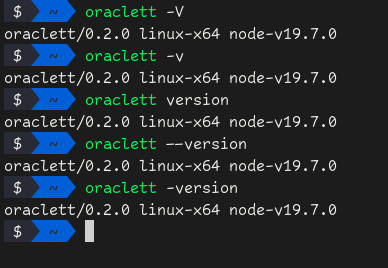
\includegraphics[scale=0.5]{demo-versions.png}
  \end{figure}
\end{frame}

\begin{frame}
  \frametitle{Flaggen anstatt Argumenten}

  \begin{figure}[H]
    \centering
    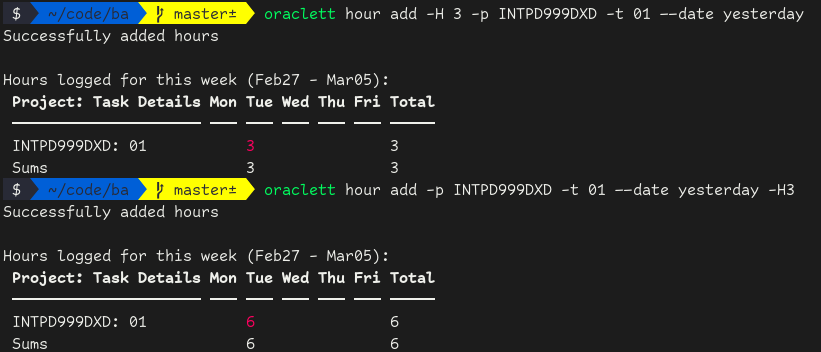
\includegraphics[scale=0.38]{demo-flags-over-args.png}
  \end{figure}
\end{frame}

\begin{frame}
  \frametitle{Relevante Standartwerte}

  \begin{figure}[H]
    \centering
    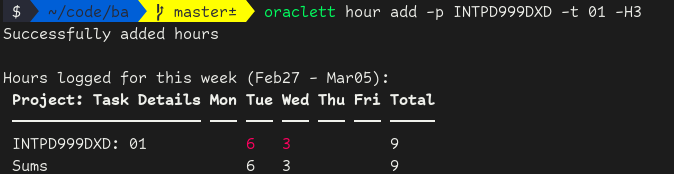
\includegraphics[scale=0.4]{demo-defaults.png}
  \end{figure}
\end{frame}

\begin{frame}
  \frametitle{Interaktives Nachfragen bei fehlendem Parameter}

  \begin{figure}[H]
    \centering
    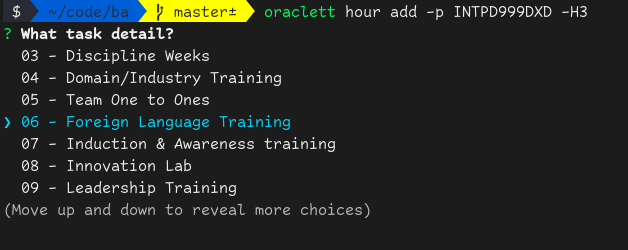
\includegraphics[scale=0.5]{demo-interactive-question.png}
  \end{figure}
\end{frame}

\begin{frame}
  \frametitle{Fehlerkorrektur}

  \begin{figure}[H]
    \centering
    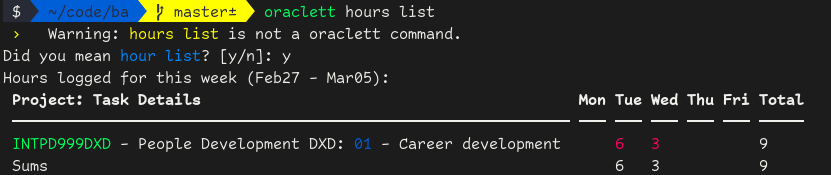
\includegraphics[scale=0.38]{demo-error-correction.png}
  \end{figure}
\end{frame}

\begin{frame}
  \frametitle{Natürliche Sprache}

  \begin{figure}[H]
    \centering
    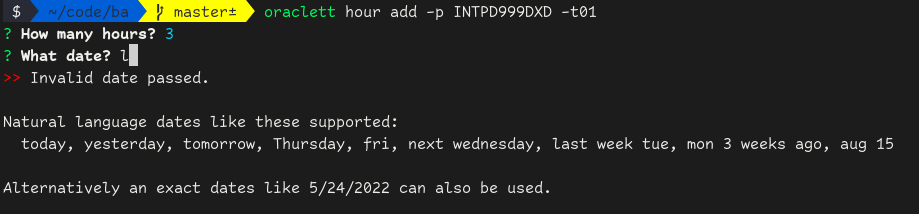
\includegraphics[scale=0.31]{demo-natural-lang.png}
  \end{figure}
\end{frame}

\begin{frame}
  \frametitle{Relevante Kommandovorschläge}

  \begin{figure}[H]
    \centering
    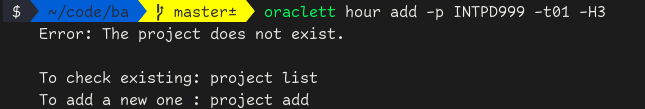
\includegraphics[scale=0.48]{demo-command-recommendations.png}
  \end{figure}
\end{frame}

\begin{frame}
  \frametitle{Autovervollständigung}

  Nicht implementiert.

  \begin{figure}[H]
    \centering
    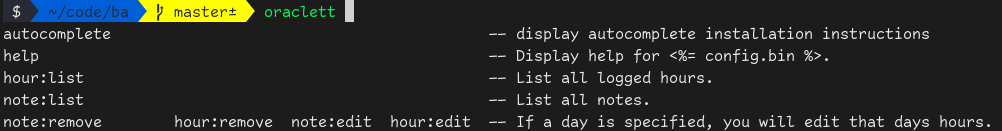
\includegraphics[scale=0.31]{apps-autocomplete.png}
  \end{figure}
\end{frame}

\begin{frame}
  \frametitle{Menü-basiertes Interface}

  Nicht implementiert.

  \begin{figure}[H]
    \centering
    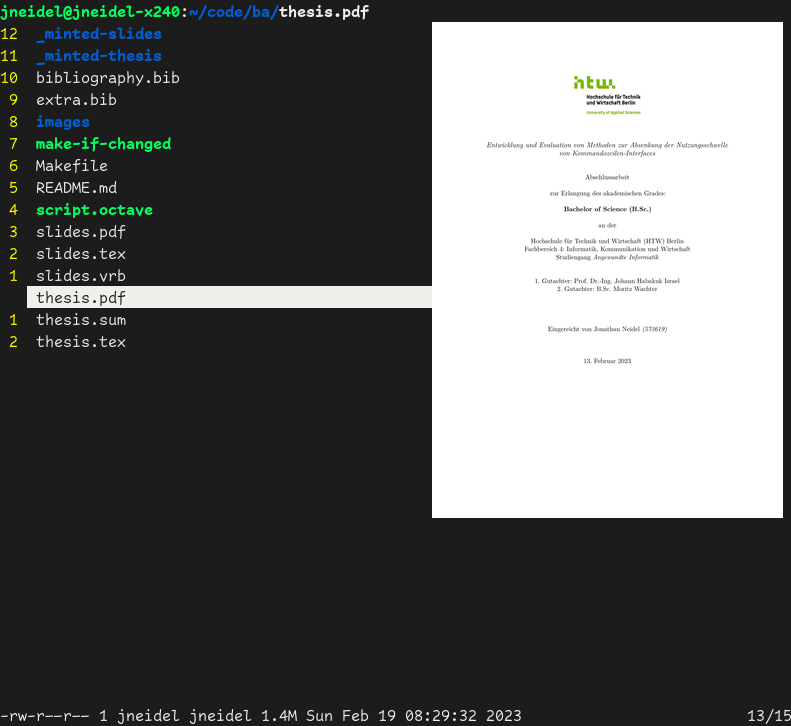
\includegraphics[scale=0.22]{demo-lf-menu.png}
    \caption{Am Beispiel von lf.}
  \end{figure}
\end{frame}

\section{Ergebnisse der Evaluation}
\begin{frame}
  \begin{center}
    {\Huge Ergebnisse der Evaluation}
  \end{center}
\end{frame}

\begin{frame}
  \frametitle{Demonstration der GUI}

  \begin{figure}[H]
    \centering
    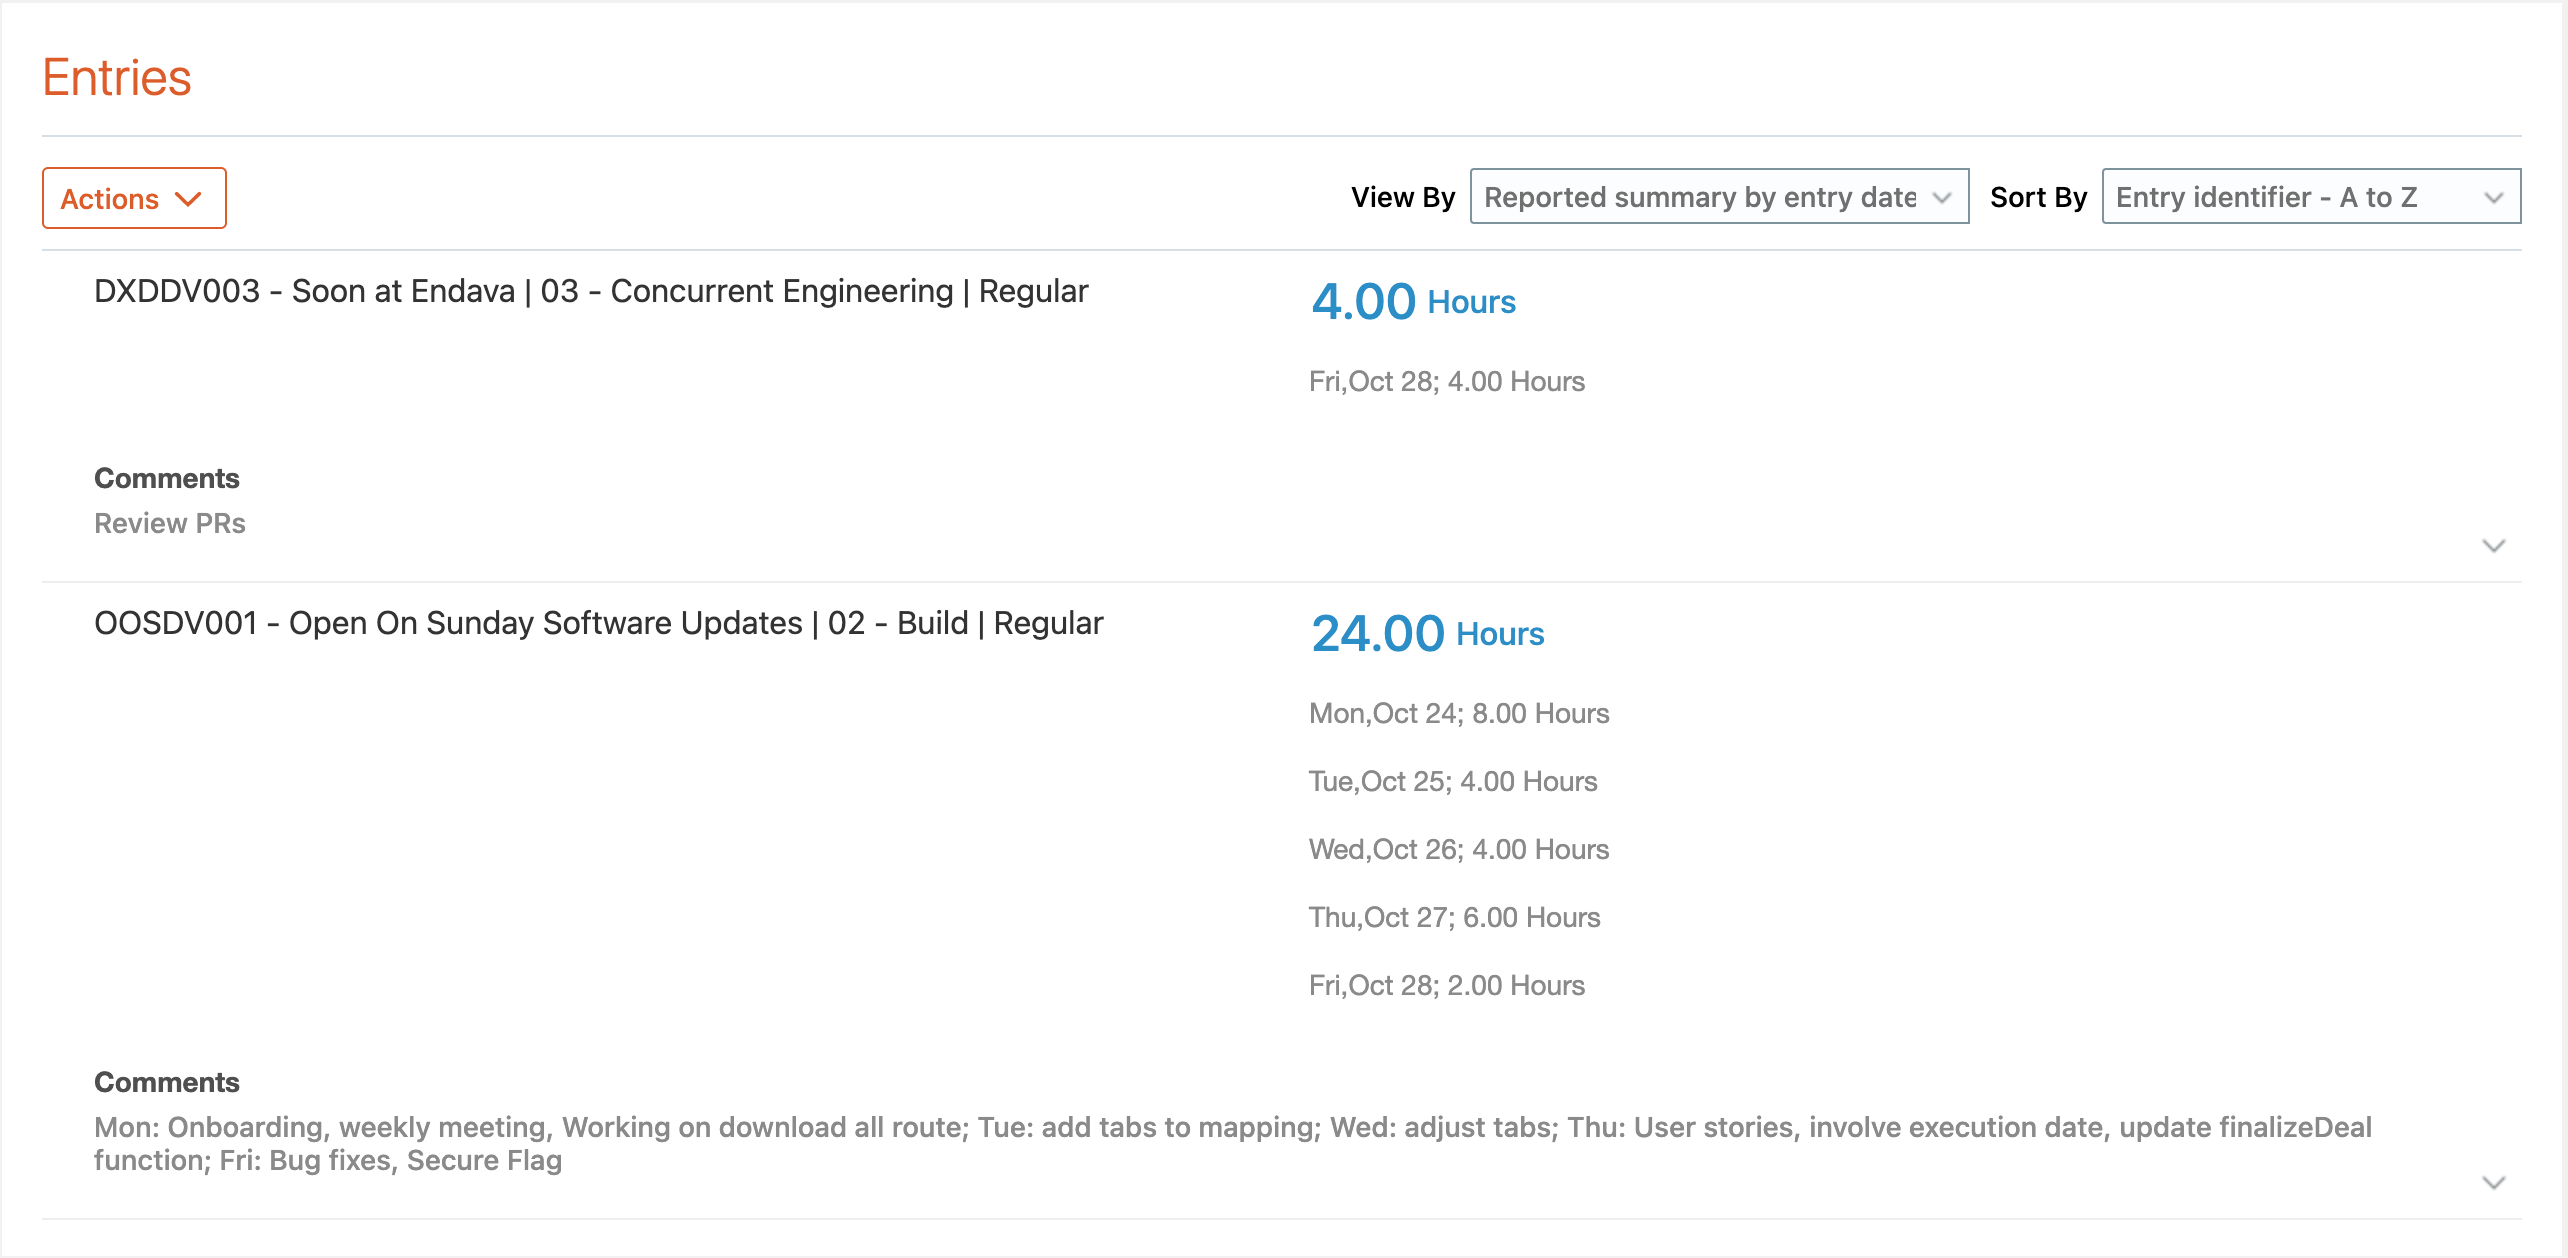
\includegraphics[scale=0.19]{oracle-real.png}
  \end{figure}
\end{frame}

\begin{frame}
  \frametitle{Hypothesen}

  \begin{enumerate}
    \item Vergleichbare Performance
    \item CLI Performance verbessert sich
    \item CLI wird vorgezogen
  \end{enumerate}

  % - Das CLI hat im Durchschnitt eine ähnliche Performance wie das GUI.
  % - Die Performance des CLI verbessert sich im Verlaufe der Aufgaben.
  % - Das CLI wird dem GUI subjektiv vorgezogen.
\end{frame}

\begin{frame}
  \frametitle{Performance}

  \begin{figure}
    \centering
    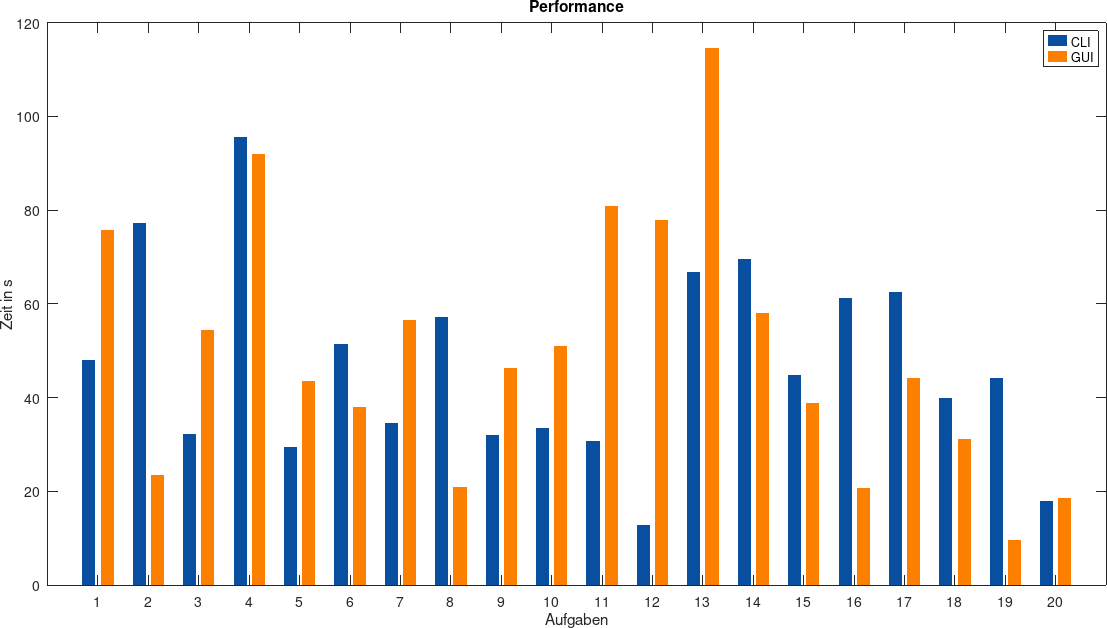
\includegraphics[scale=0.28]{performance.png}
  \end{figure}
\end{frame}

\begin{frame}
  \frametitle{Performance Unterschiede}

  \begin{figure}[H]
    \centering
    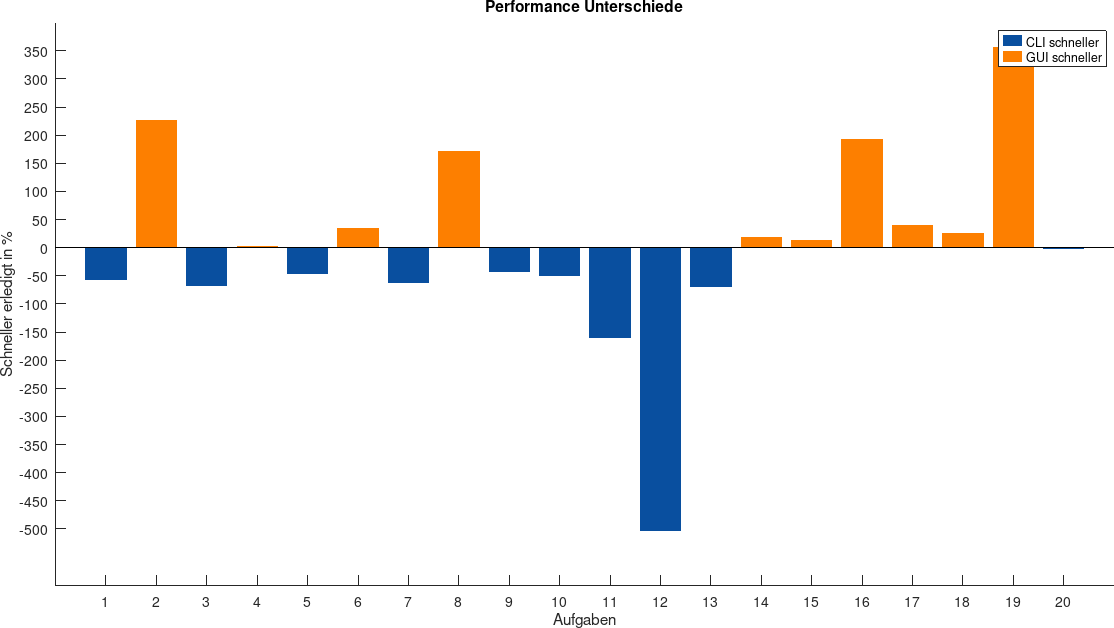
\includegraphics[scale=0.28]{performance-diff.png}
  \end{figure}
\end{frame}

\begin{frame}
  \frametitle{CLI Performance}

  \begin{figure}[H]
    \centering
    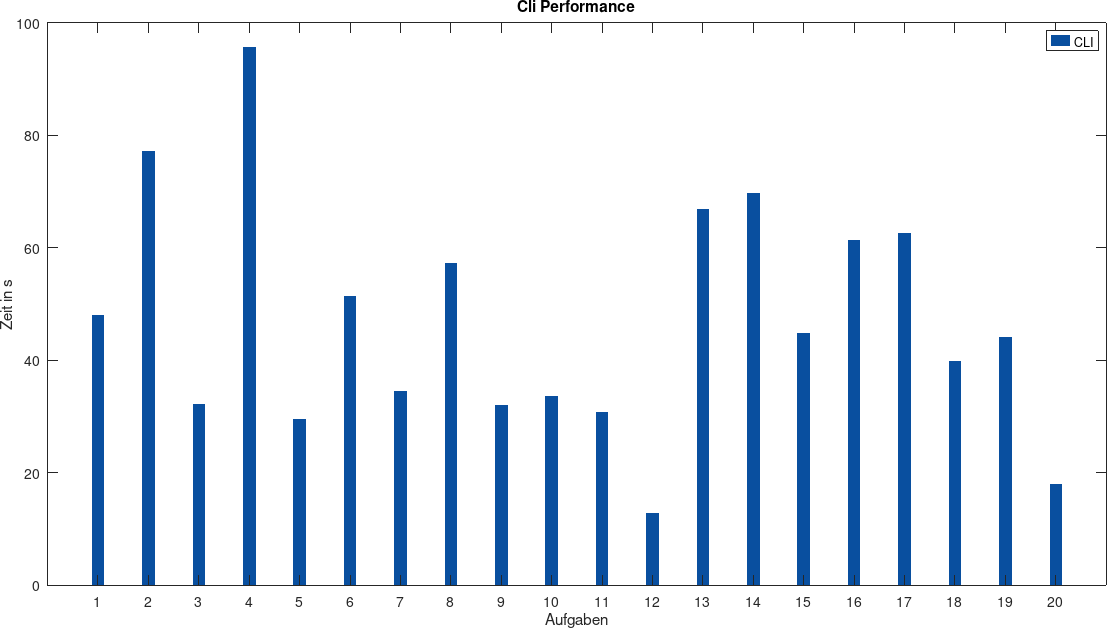
\includegraphics[scale=0.28]{performance-cli.png}
  \end{figure}
\end{frame}

\begin{frame}
  \frametitle{Umfrage I}

  \begin{figure}
    \centering
    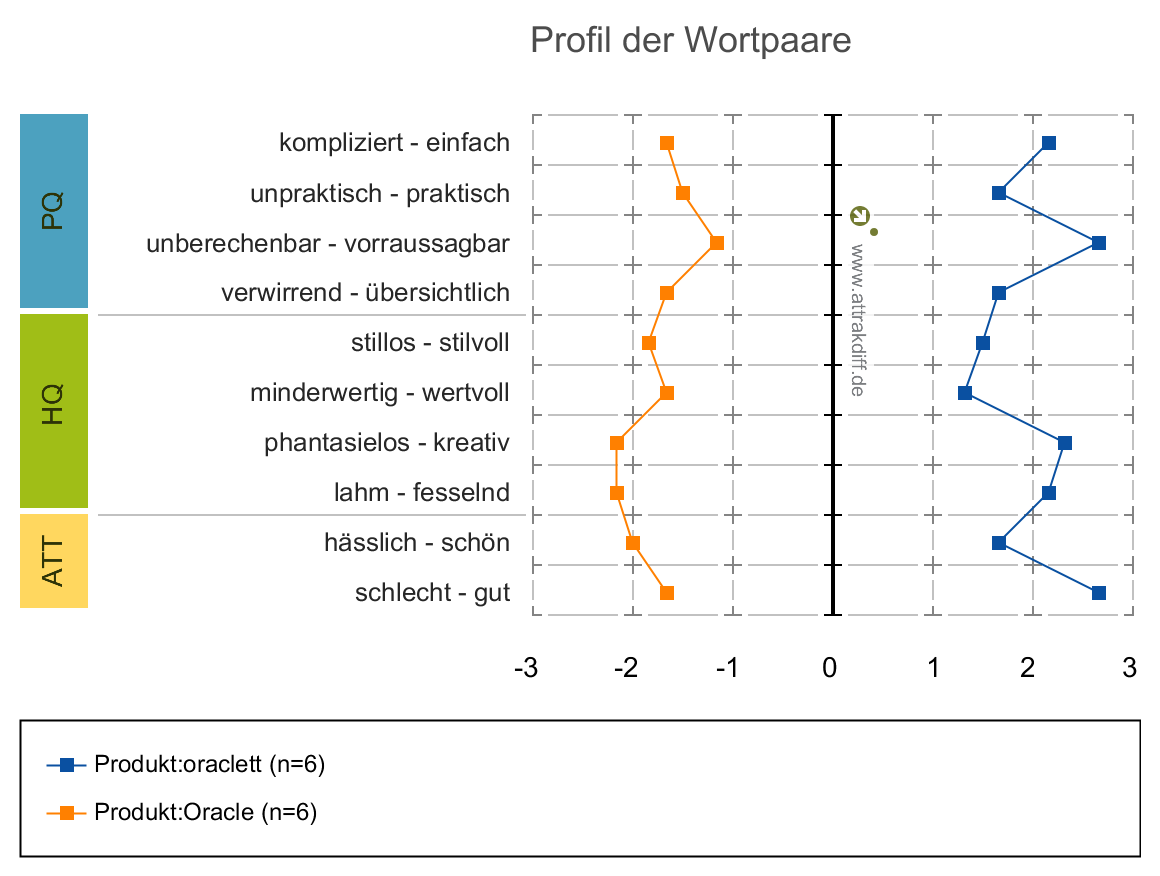
\includegraphics[scale=0.3]{attrak-wortpaare.png}
  \end{figure}
\end{frame}

\begin{frame}
  \frametitle{Umfrage II}

\begin{figure}
  \centering
  \begin{minipage}[b]{0.4\textwidth}
    \centering
    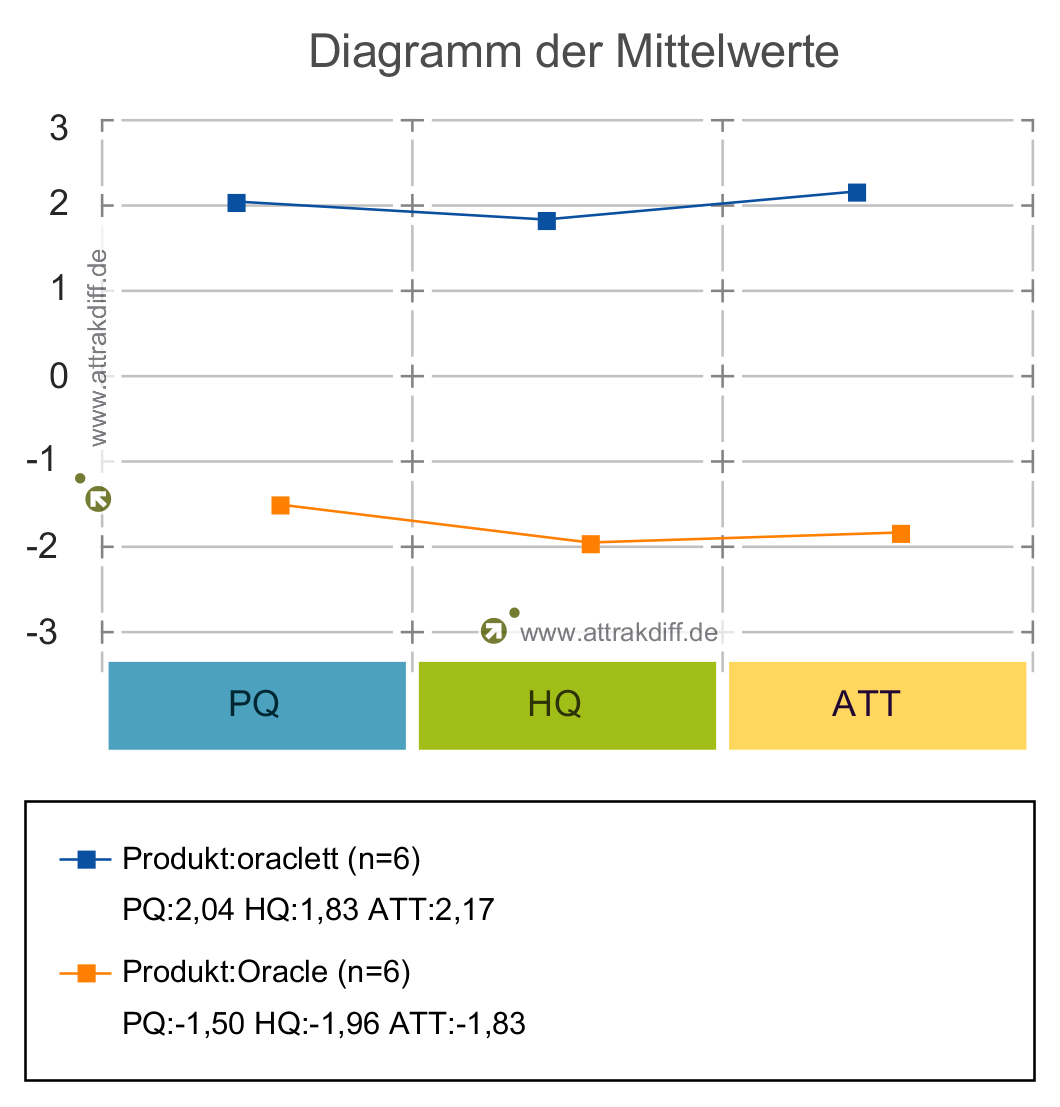
\includegraphics[scale=0.19]{attrak-mittelwerte.png}
  \end{minipage}
  \hfill
  \begin{minipage}[b]{0.4\textwidth}
    \centering
    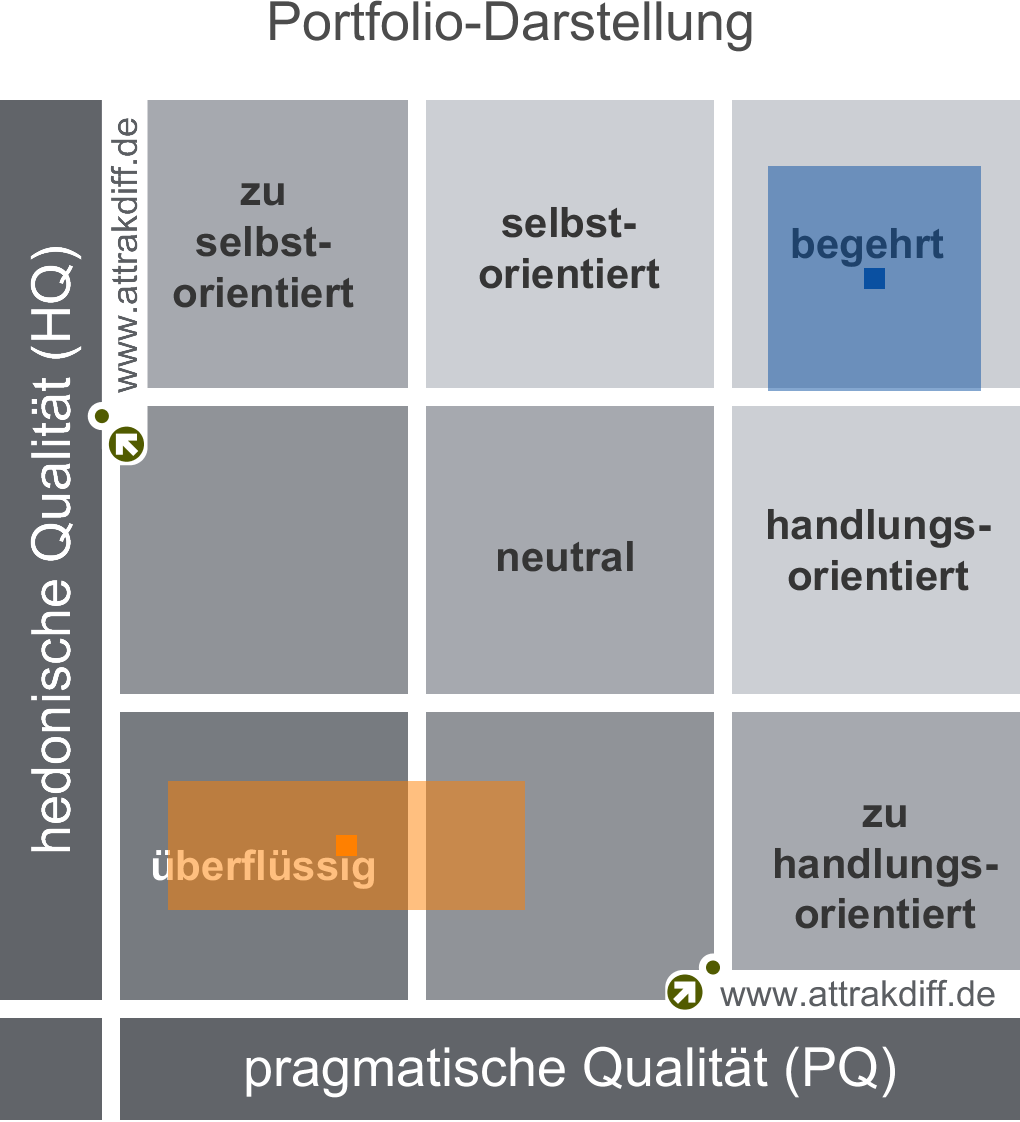
\includegraphics[scale=0.18]{attrak-portfolio.png}
  \end{minipage}
\end{figure}
\end{frame}

\section{Fazit}
\begin{frame}
  \begin{center}
    {\Huge Fazit}
  \end{center}
\end{frame}

\end{document}

